\documentclass{beamer}
\usepackage{hyperref}
\usetheme{Madrid}
\usepackage{graphicx}
\usepackage{xcolor} 
\usepackage{fouriernc}
\usepackage{tgschola}
\title{}
\author{Nithin}
\institute{}
\date{\today}
\begin{document}
	\section{Nature of Light}
\begin{frame}{Test}
\href{https://www.youtube.com/watch_popup?v=xpcX3B4xE7Q}{Lenses}
\end{frame}

\begin{frame}
	
 \frametitle{Ray Model of Light}
 3 ways light can travel from a source to another location
 	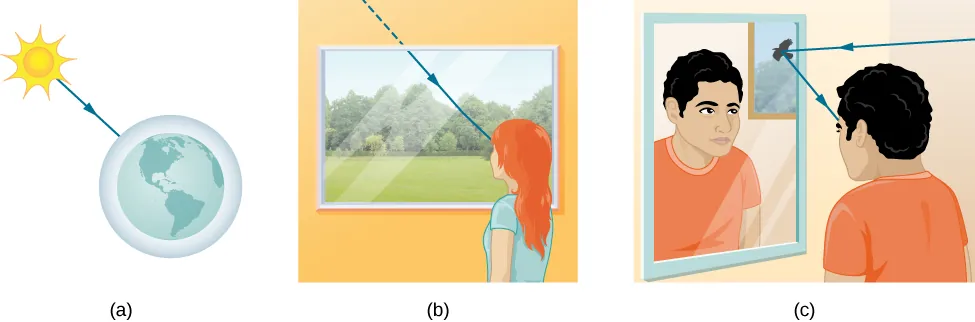
\includegraphics[width=10cm,height=3cm]{1.png}
 \begin{enumerate}
 	\item[a] directly from source through vaccum . Sun to Earth
 	\item[b] light can travel through various media like Air, glass, water to the observer 
 	\item[c] light can also arrive after being reflected such as mirrors
 \end{enumerate}

\end{frame}
\begin{frame}
\begin{block}{Ray of Light}
	We model path of light as a straight line called \alert{ray}
\end{block}
\begin{itemize}
	\item Light behaves both as a particle and a wave
	\item When light interacts with an object several times larger than its wavelength($\approx 10^{-6}$), it travels in a straight line and acts like a ray.
	\item Light may change direction when it 
	\begin{itemize}
		\item reflection : encounters objects (such as a mirror) 
		\item refraction: passing from one material to another (such as in passing from air to glass) 
	\end{itemize}	
\end{itemize}
\end{frame}

\begin{frame}{Law of Reflection}
	\begin{block}{Law of Reflection}
		the law states that agle of reflection is equal to angle of incidence
		\begin{displaymath}
			\theta_{r} = \theta_{i}
		\end{displaymath}
	\end{block}
	\begin{center}
		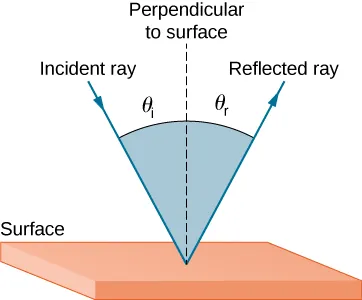
\includegraphics[width=5cm, height=5cm]{2.png}
	\end{center}
\end{frame}

\begin{frame}
	\frametitle{Reflections}
	\begin{center}
		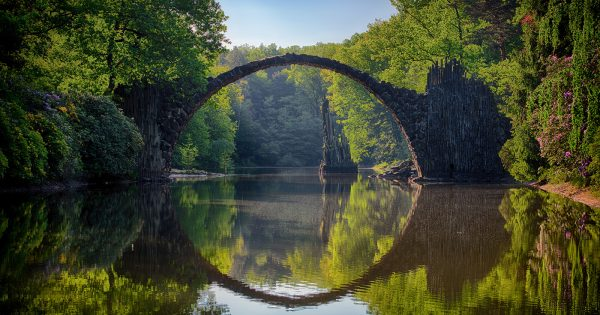
\includegraphics[scale=0.8]{3.jpg}	
	\end{center}
\end{frame}

\begin{frame}
	\frametitle{Reflections}
	\begin{enumerate}
		\pause
		\item Specular Reflection 
		 \pause
		\item Diffused Reflection  
	\end{enumerate}
\end{frame}


\end{document}
